\documentclass[11pt]{article}

\usepackage[margin=1.7cm,top=2.5cm,bottom=2cm,letterpaper]{geometry}
\usepackage{enumitem}
\usepackage{tikz}
\usepackage{mathpazo}
\usepackage{times}
\usepackage[document]{ragged2e}
\usepackage[none]{hyphenat}
\usepackage{siunitx}
\usepackage{multicol}
\usepackage{fancyhdr}

\sisetup{number-math-rm=\mathnormal}

%\renewcommand{\familydefault}{\sfdefault}

\newcommand{\pic}[2]{\includegraphics[width=#1\textwidth]{#2}}

\setlength{\parindent}{0pt}
\setlength{\headheight}{14pt}
\begin{document}

\pagestyle{fancy}
\lhead{Student Number:}
\chead{}
\rhead{Name:\hspace{2in}}
\lfoot{}\cfoot{-\textsf{\textbf{\thepage}}-}
\rfoot{\textsf{\textbf{GO ON TO THE NEXT PAGE.}}}

\begin{center}
  \vspace{-.35in}
  {\large
    \textbf{AP PHYSICS C: ELECTROSTATICS AND \& GAUSS'S LAW}
  }
\end{center}

\textbf{Directions:} Each of the questions or incomplete statements below is
followed by five suggested answers or\\
completions. Select the one that is best
in each case and place the letter of your choice in the corresponding box on
the student answer sheet.

\vspace{10pt}\textbf{Note:} To simplify calculations, you may use
$g=\SI{10}{m/s^2}$ in all problems.

\raggedcolumns
\begin{multicols}{2}
  \begin{enumerate}[leftmargin=18pt]

  \item Two electric objects experience a repulsive force. What happens to that
    force if the distance between the objects is doubled?
    \begin{enumerate}[noitemsep,topsep=0pt,leftmargin=18pt,label=(\Alph*)]
    \item It decreases to one-fourth its value.
    \item It decreases to one-half its value.
    \item It stays the same.
    \item It doubles.
    \item It quadruples.
    \end{enumerate}

  \item A pith ball is a tiny piece of Styrofoam that is covered with a
    conductive paint. One pith ball initially has a charge of \SI{6.4e-8}{C},
    and it touches an identical, neutral pith ball. After the pith balls are
    separated, what is the charge on the pith ball that had the initial charge?
    \begin{enumerate}[noitemsep,topsep=0pt,leftmargin=18pt,label=(\Alph*)]
    \item\SI{6.4e-8}{C}
    \item\SI{3.2e-8}{C}
    \item\SI{0}{C}
    \item\SI{-3.2e-8}{C}
    \item\SI{-6.4e-8}{C}
    \end{enumerate}

  \item Glass becomes positively charged when it is rubbed with silk. Which
    of the following is the best description of what’s happening?
    \begin{enumerate}[noitemsep,topsep=0pt,leftmargin=18pt,label=(\Alph*)]
    \item Electrons are rubbed off the glass onto the silk.
    \item Electrons are rubbed off the silk onto the glass.
    \item Protons are rubbed off the glass onto the silk.
    \item Protons are rubbed off the silk onto the glass.
    \item Neutrons in the glass have an affinity for positive charge.
    \end{enumerate}
  
  \item Consider an isolated, neutral system consisting of wool fabric and a
    rubber rod. If the rubber rod is rubbed with wool to become negatively
    charged, what can be said about the wool fabric?
    \begin{enumerate}[noitemsep,topsep=0pt,leftmargin=18pt,label=(\Alph*)]
    \item It becomes equally negatively charged.
    \item It becomes equally positively charged.
    \item It becomes negatively charged but not equally.
    \item It becomes positively charged but not equally.
    \item In a neutral system, neither object can become charged.
    \end{enumerate}
    \columnbreak
  \item An electron and a proton are separated by \SI{1.50e-10}{m}. If they are
    released, which one will accelerate at a greater rate, and what is the
    magnitude of that acceleration?
    \begin{enumerate}[noitemsep,topsep=0pt,leftmargin=18pt,label=(\Alph*)]
    \item The electron; \SI{1.12e22}{m/s^2}
    \item The proton; \SI{1.12e22}{m/s^2}
    \item The electron; \SI{6.13e18}{m/s^2}
    \item The proton; \SI{6.13e18}{m/s^2}
    \item They both accelerate at the same rate; \SI{1.02e-8}{m/s^2}
    \end{enumerate}

    \begin{center}
      \begin{tikzpicture}[scale=3]
        \draw[dashed](0,0)--(1,0)--(.5,.866)--cycle;
        \draw[fill=black](.5,.289) circle(0.03);
        \draw[fill=white](0,0) circle(0.05) node[left]{$+Q\;$};
        \draw[fill=white](1,0) circle(0.05) node[right]{$\;-Q$};
        \draw[fill=white](.5,.866) circle(0.05) node[right]{$\;2Q$};
      \end{tikzpicture}
    \end{center}
    
  \item\vspace{-.2in} Three charges, $+Q$, $−Q$, and $+2Q$, are arranged in an
    equilateral triangle as shown. Which of the arrows below best represents
    the direction of the electric field at the center of the triangle?
  
    \begin{enumerate}[noitemsep,topsep=0pt,leftmargin=18pt,label=(\Alph*)]
    \item $\displaystyle\downarrow$
    \item $\displaystyle\uparrow$
    \item $\displaystyle\searrow$
    \item $\displaystyle\swarrow$
    \item $\displaystyle\nearrow$
    \end{enumerate}

  \item The potential $V$ as a function of distance $r$ for a particular charge
    distribution is given by the equation $V=ar^{-1}$. The electric field as
    a function of distance $r$ from the charge distribution is
    \begin{enumerate}[noitemsep,topsep=0pt,leftmargin=18pt,label=(\Alph*)]
    \item $1/3\;ar^{-3}$
    \item $2ar^{-1}$
    \item $ar^{−2}$
    \item $−a(\ln r)$
    \item $−ar^{-2}$
    \end{enumerate}

    \columnbreak

    \hspace{-18pt}\textbf{Questions 8 and 9}

    \vspace{-.2in}
    \begin{center}
      \begin{tikzpicture}[scale=3]
        \draw[dashed](0,0)--(1,0)--(1,1) node[midway,right]{$a$}
        --(0,1)--cycle;
        \draw[fill=black](.5,.5) circle(0.03);
        \draw[fill=white](0,0) circle(0.05) node[below left]{$q$};
        \draw[fill=white](1,0) circle(0.05) node[below right]{$q$};
        \draw[fill=white](0,1) circle(0.05) node[above left]{$q$};
        \draw[fill=white](1,1) circle(0.05) node[above right]{$q$};
      \end{tikzpicture}
    \end{center}
    
  \item\vspace{-.3in} Four charges are arranged at the corners of a square of
    side a as shown. Which of the following is true of the electric field and
    the electric potential at the center of the square?
    
    \begin{tabular}{rll}
        & \underline{Electric Field} & \underline{Electric Potential}\\
      (A) & zero & zero \\
      (B) & $\frac{kQ}{a\sqrt{2}}$ & zero \\
      (C) & $\frac{kQ^2}{2a^2}$ &  $\frac{kQ}{2a}$\\
      (D) & zero &  $\frac{kQ}{\sqrt{2a}}$\\
      (E) & $\frac{kQ^2}{2a}$ & $\frac{kQ}{a\sqrt{2}}$
    \end{tabular}
    \columnbreak
    
  \item\vspace{-.1in} Which of the following diagrams best represents how you might rearrange
    the charges so that the electric field at the center would point directly
    toward the top of the page?
    \begin{enumerate}[noitemsep,topsep=0pt,leftmargin=18pt,label=(\Alph*)]
    \item\vspace{-.1in}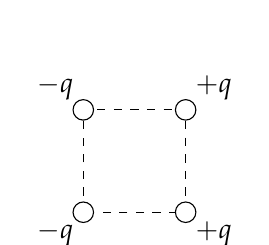
\begin{tikzpicture}[scale=1.3]
      \draw[dashed](0,0) rectangle(1,1);
      \draw[fill=white](0,0) circle(0.1) node[below left]{$-q$};
      \draw[fill=white](1,0) circle(0.1) node[below right]{$+q$};
      \draw[fill=white](0,1) circle(0.1) node[above left]{$-q$};
      \draw[fill=white](1,1) circle(0.1) node[above right]{$+q$};
    \end{tikzpicture}
    \item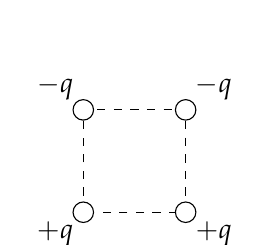
\begin{tikzpicture}[scale=1.3]
      \draw[dashed](0,0) rectangle(1,1);
      \draw[fill=white](0,0) circle(0.1) node[below left]{$+q$};
      \draw[fill=white](1,0) circle(0.1) node[below right]{$+q$};
      \draw[fill=white](0,1) circle(0.1) node[above left]{$-q$};
      \draw[fill=white](1,1) circle(0.1) node[above right]{$-q$};
    \end{tikzpicture}
    \item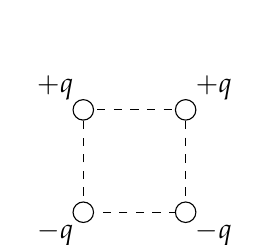
\begin{tikzpicture}[scale=1.3]
      \draw[dashed](0,0) rectangle(1,1);
      \draw[fill=white](0,0) circle(0.1) node[below left]{$-q$};
      \draw[fill=white](1,0) circle(0.1) node[below right]{$-q$};
      \draw[fill=white](0,1) circle(0.1) node[above left]{$+q$};
      \draw[fill=white](1,1) circle(0.1) node[above right]{$+q$};
    \end{tikzpicture}
    \item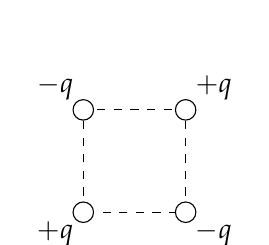
\begin{tikzpicture}[scale=1.3]
      \draw[dashed](0,0) rectangle(1,1);
      \draw[fill=white](0,0) circle(0.1) node[below left]{$+q$};
      \draw[fill=white](1,0) circle(0.1) node[below right]{$-q$};
      \draw[fill=white](0,1) circle(0.1) node[above left]{$-q$};
      \draw[fill=white](1,1) circle(0.1) node[above right]{$+q$};
    \end{tikzpicture}
    \item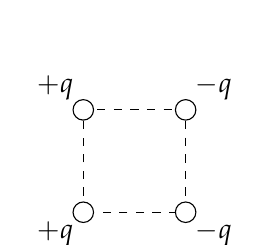
\begin{tikzpicture}[scale=1.3]
      \draw[dashed](0,0) rectangle(1,1);
      \draw[fill=white](0,0) circle(0.1) node[below left]{$+q$};
      \draw[fill=white](1,0) circle(0.1) node[below right]{$-q$};
      \draw[fill=white](0,1) circle(0.1) node[above left]{$+q$};
      \draw[fill=white](1,1) circle(0.1) node[above right]{$-q$};
    \end{tikzpicture}
    \end{enumerate}

  \item A nonconducting sphere does not have a uniform charge density, but the
    density $\rho$ varies with the distance $r$ from the center of the sphere
    according to the equation $\rho=\beta r$ where $\beta$ is a positive
    constant. The electric field inside the sphere ($r<R$) at a distance $r$
    from the center of the sphere is
    \begin{enumerate}[noitemsep,topsep=0pt,leftmargin=18pt,label=(\Alph*)]
    \item $\displaystyle\frac{\beta r^2}{12\epsilon_0}$
    \item $\displaystyle\frac{\beta r^3}{3\epsilon_0}$
    \item $\displaystyle\frac{\beta r}{2\epsilon_0}$
    \item $\displaystyle\frac{\beta r^2}{2\epsilon_0}$
    \item $\displaystyle\frac{\beta r^2}{4\epsilon_0}$
    \end{enumerate}
    \columnbreak
    
  \item The electric potential at the surface of the sphere from the last
    question is
    \begin{enumerate}[noitemsep,topsep=0pt,leftmargin=18pt,label=(\Alph*)]
    \item $\displaystyle\frac{\beta R^3}{4\epsilon_0}$
    \item $\displaystyle\frac{\beta R}{2\epsilon_0}$
    \item $\displaystyle\frac{\beta R^3}{3\epsilon_0}$
    \item $\displaystyle\frac{\beta R^2}{2\epsilon_0}$
    \item $\displaystyle\frac{\beta R^2}{4\epsilon_0}$
    \end{enumerate}
  \item According to Gauss's law, the net electric flux passing through a closed
    surface is
    \begin{enumerate}[noitemsep,topsep=0pt,leftmargin=18pt,label=(\Alph*)]
    \item positive if the flux is entering the surface
    \item negative if the flux is exiting the surface
    \item positive if the net charge inside the surface is zero
    \item negative if the net charge inside the surface is zero
    \item zero if the net charge inside the surface is zero
    \end{enumerate}

  \item According to Gauss's law, which of the following statements is true?
    \begin{enumerate}[noitemsep,topsep=0pt,leftmargin=18pt,label=(\Alph*)]
    \item It is possible to have a nonzero electric field, but zero electric
      flux.
    \item It is possible to have a nonzero electric flux, but zero electric
      field.
    \item It is possible to have a nonzero electric flux through a closed
      surface even if the enclosed charge in a surface is zero.
    \item If a surface is not closed (such as a sheet of paper), the flux
      through it must be zero.
    \item It is possible for charges located outside a closed surface to produce
      a net positive flux through the surface.
    \end{enumerate}
    
  \item Electric potential
    \begin{enumerate}[noitemsep,topsep=0pt,leftmargin=18pt,label=(\Alph*)]
    \item is a vector quantity that depends on the direction of the electric
      field
    \item is a scalar quantity that depends on the magnitude and sign of charges
      in the vicinity
    \item is a scalar quantity that depends on the square of the distance from
      the charges in the vicinity
    \item is a vector quantity that depends on the sign of the charges in the
      vicinity
    \item is a vector quantity that must point from high to low potential
    \end{enumerate}

    \begin{center}
      \pic{.3}{cube.png}
    \end{center}
  
  \item\vspace{-.2in} A cube has sides of length $a$. The cube rests so that one
    side rests on
    the $x$-axis as shown. An electric field is established in the $x$-direction
    according to the function $E_x=bx^2$ , where $b$ is a positive constant.
    Which of the following statements is true?
    
    \begin{enumerate}[noitemsep,topsep=0pt,leftmargin=18pt,label=(\Alph*)]
    \item There is a net charge inside the cube.
    \item There is no net charge inside the cube.
    \item The flux passing through the cube is negative.
    \item The flux passing through the cube is zero.
    \item The flux diminishes while passing through the cube.
    \end{enumerate}

  \item The charge inside the cube from the previous question can be expressed
    by the equation
    \begin{enumerate}[noitemsep,topsep=0pt,leftmargin=18pt,label=(\Alph*)]
    \item $\epsilon_0ba$
    \item $\epsilon_0ba^2$
    \item $\epsilon_0ba^3$
    \item $\epsilon_0ba^4$
    \item $\epsilon_0b^22a^2$
    \end{enumerate}

  \item Gauss's law is most convenient to use when calculating an electric field
    due to
    \begin{enumerate}[noitemsep,topsep=0pt,leftmargin=18pt,label=(\Alph*)]
    \item charges outside a closed surface
    \item charges inside a closed surface that has high symmetry
    \item charges inside a closed surface that has low symmetry
    \item a potential difference that is negative
    \item a potential difference that is positive
    \end{enumerate}
    \columnbreak
    
  \item Which of the following statements is true of electric field and
    equipotential lines?
    \begin{enumerate}[noitemsep,topsep=0pt,leftmargin=18pt,label=(\Alph*)]
    \item The electric field vector always points in the same direction as the
      equipotential lines.
    \item The electric field always points in the opposite direction of the
      equipotential lines.
    \item The electric field always points perpendicular to the equipotential
      lines.
    \item The electric field is always equal to the equipotential lines.
    \item Equipotential lines always form a circle around electric field lines.
    \end{enumerate}

    \columnbreak
    \columnbreak
    \begin{center}
      \begin{tikzpicture}[scale=1.3]
        \draw (0,0) ellipse (0.7 and 1.3);
        \draw[->](0,0)--(0,1.3) node[midway,right]{R};
        \draw[dashed](0,0)--(0,-1.3);
        \draw[dashed](-3.2,0)--(3.2,0);
        \foreach \x in {-3,-2,-1,1,2,3}{
          \draw(\x,-.2)--(\x,.2) node[pos=0,below] {$\x d$};
        }
      \end{tikzpicture}
    \end{center}

  \item A positively charged ring of radius R is made of conducting material and
    has a charge $Q$ distributed uniformly around it. The center of the ring is
    located at point 0 on the $x$-axis. The potential $V$ at a distance $3d$
    from point 0 on the $x$-axis is
    \begin{enumerate}[noitemsep,topsep=0pt,leftmargin=18pt,label=(\Alph*)]  
    \item $\displaystyle V=\frac{kQ}{9d^2}$
    \item $\displaystyle V=\frac{kQ}{3d^2}$
    \item $\displaystyle V=\frac{kQ}{R^2+9d^2}$
    \item $\displaystyle V=\sqrt{\frac{kQ}{R^2+9d^2}}$
    \item $\displaystyle V=\frac{kQ}{\sqrt{R^2+9d^2}}$
    \end{enumerate}
  \end{enumerate}
  \columnbreak
\end{multicols}

\newpage
\begin{center}
  \textbf{
    PHYSICS C: MECHANICS\\
    SECTION II\\
    5 Questions}
\end{center}

\textbf{Directions:} Answer all questions. The suggested time is about 15
minutes for answering each of the questions, which are worth 15 points each.
The parts within a question may not have equal weight. All final numerical
answers should include appropriate units. Credit depends on the quality of your
solutions and explanations, so you should show your work. Credit also depends
on demonstrating that you know which physical principles would be appropriate
to apply in a particular situation. Therefore, you should clearly indicate
which part of a question your work is for.


\begin{enumerate}[leftmargin=15pt]

\item Two identical small spheres of mass $m$ are suspended from a common point
  by threads of length L. When each sphere carries a charge $q$, each thread
  makes an angle $\theta$ with the vertical as shown in the figure below.
  (a) Express charge $q$ in terms of $\theta$, $m$, $L$ and any other relevant
  constants, and (b) Compute $q$ if $m=\SI{10}{\gram}$, $L=\SI{50}{cm}$ and
  $\theta=\ang{10}$.
  
  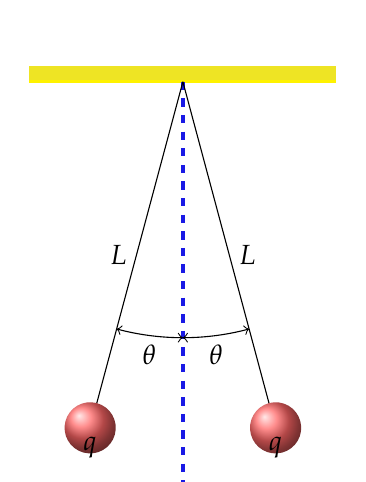
\begin{tikzpicture}[scale=1.3]
    \tikzstyle{balloon}=[ball color=red!60];
    \fill[yellow!85!gray](-1.5,0) rectangle(1.5,0.15);
    \draw[very thick,yellow](-1.5,0)--(1.5,0);
    \draw[dashed,very thick,blue!80!gray](0,0)--(0,-4);
    \draw[<->](0,-2.5) arc (270:285:2.5) node[midway,below]{$\theta$};
    \draw[<->](0,-2.5) arc (270:255:2.5) node[midway,below]{$\theta$};
    \begin{scope}[rotate=15]
      \draw(0,0)--(0,-3.5) node[midway,right]{$L$};
      \shade[balloon] (0,-3.5) circle (0.25) node[below]{$q$};
    \end{scope}
    \begin{scope}[rotate=-15]
      \draw(0,0)--(0,-3.5) node[midway,left]{$L$};
      \shade[balloon] (0,-3.5) circle (0.25) node[below]{$q$};
    \end{scope}
  \end{tikzpicture}
  \vspace{1.35in}
  
\item Five equal charges $Q$ are equally spaced on a semicircle or radius $R$
  as shown in the figure below. Find the force on a charge $q$ located at the
  centerof the semicircle.
  
  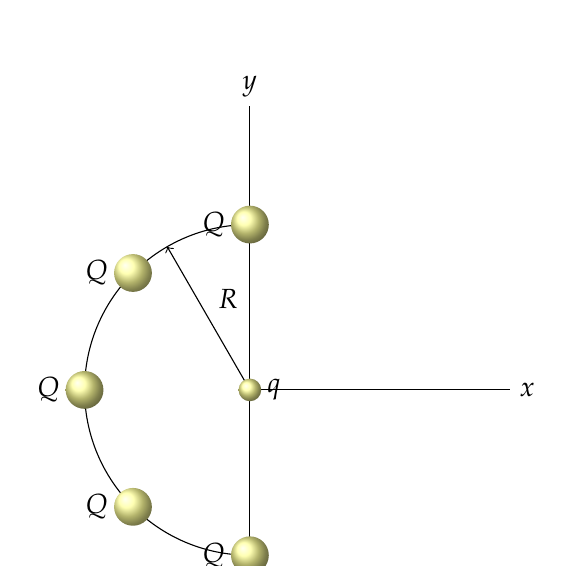
\begin{tikzpicture}[scale=1.2]
    \tikzstyle{balloon}=[ball color=yellow!40];
    \draw(0,-1.75)--(0,3) node[pos=1,above]{$y$};
    \draw(0,0)--(2.75,0) node[pos=1,right]{$x$};
    \draw[->,rotate=120](0,0)--(1.75,0) node[midway,above right]{$R$};
    \draw(0,1.75) arc (90:270:1.75);
    \foreach \x in {0,45,...,180}
    \shade[balloon,rotate=\x] (0,1.75) circle (0.2) node[left]{$Q\;\;$};
    \shade[balloon] (0,0) circle(0.12) node[right]{$\;q$};
  \end{tikzpicture}
  \newpage
\item Two positive charges $+q$ are on the $y$ axis at $y=+a$ and $y=-a$.
  \begin{enumerate}[noitemsep]
  \item Show that the electric field on the $x$ axis is along the $x$ axis with
    $E_x=2kqx(x^2+a^2)^{-3/2}$.
  \item Show that near the origin, when $x\ll a$, $E_x\approx 2kqx/a^3$.
  \item Show that for $x\gg a$, $E_x\approx 2kq/x^2$.
  \item Explain why you should expect the result in (c) even before calculating
    it.
  \end{enumerate}
  A bead of mass $m$ with a negative charge $-q$ slides along a thread that
  runs along the $x$ axis.
  \begin{enumerate}[noitemsep]
  \item Show that for small displacements $x\ll a$, the bead experiences a
    restoring force that is proportional to $x$ and therefore undergoes
    simple harmonic motion.
  \item Find the period of the motion.
  \end{enumerate}
  \newpage

\item Using Gauss's law, find
  \begin{enumerate}
  \item the electric field strength inside and outside of a uniformly charged
    hollow sphere of radius $R$ and surface charge density $\sigma$ (charge
    per unit area).

  \item the electric field inside and outside an infinitely long cyclindrical
    shell of charge of radius $R$ with charge discibution $\sigma$ (charge
    per unit area).
  \item the electric field strength inside and outside a infinitely long solid
    cylinder of radius $R$ carrying a linear uniform charge density $\rho$
    (charge per unit volume).
  \end{enumerate}
  Hint: In all cases, think about where to put the Gaussian surface. Take
  advantage of symmetry.
  \newpage

\item A parallel-plate capacitor has a capacitance $C_0$ and plate separation
  of $d$. To dielectric slabs of constants $\kappa_1$ and $\kappa_2$, each of
  thickness $d/2$ and having the same area as the plates, are inserted between
  the plates as shown in the figure below. When the free charge on the plates
  are $Q$,
  \begin{enumerate}[noitemsep]
  \item find the electric field in each of the dielectric
  \item find the potential difference between the plates
  \item show that the new capacitance is given by:
    $\displaystyle C=\frac{\kappa_1\kappa_2}{\kappa_1+\kappa_2}C_0$
  \end{enumerate}
  \pic{0.25}{stacked.png}
  \vspace{1.5in}

\item Several point charges produce the equipotential lines shown.
  \begin{enumerate}[noitemsep]
  \item At which point on the diagram is the magnitude of the electric field
    greatest? Explain.
  \item Points C and D are approximately \SI{0.02}{\metre} apart. Point F is
    halfway between points C and D. What is the electric field at point F?
  \item A \SI{5.0}{\micro\coulomb} point charge is moved from point C to point
    E, then to point D by an external force. Determine the work done by the
    external force.
  \end{enumerate}
  \pic{.45}{equipotentials.png}
\end{enumerate}
\end{document}
